\documentclass[11pt]{article}
\usepackage{graphicx}
\usepackage{hyperref}
\usepackage[dvipsnames, svgnames, x11names, hyperref]{xcolor}
\hypersetup{
	colorlinks,
	citecolor=Violet,
	linkcolor=Red,
	urlcolor=Blue}
\usepackage{natbib}

\setlength{\textwidth}{6.5in}
\setlength{\headheight}{0in}
\setlength{\textheight}{8.0in}
\setlength{\hoffset}{0in}
\setlength{\voffset}{0in}
\setlength{\oddsidemargin}{0in}
\setlength{\evensidemargin}{0in}


\title{Homework 5 Solution}

\author{Nana Ama Nyamekye Darpaah}

\begin{document}
	
	\maketitle
This is my GitHub link: \href{https://github.com/nnd2016/phys-ga2000.git}{Nana Ama's GitHub Link}
	
\section{Question 1}

The formula
	\begin{equation}
	f(x) = 1 + \tanh(2x) 
	\end{equation}

can be solved analytically as 
	\begin{equation}
	f'(x) = 1 - \tanh^{2}(2x) 
	\end{equation}

Plotting the analytical version and that obtained numerically from python on the range $x = [-4, 4]$, it is seen from Figure \ref{fig:analytic vs numeric} that there is little error.
\\
\begin{figure}[h]\begin{center} 
		\vspace{12pt}
		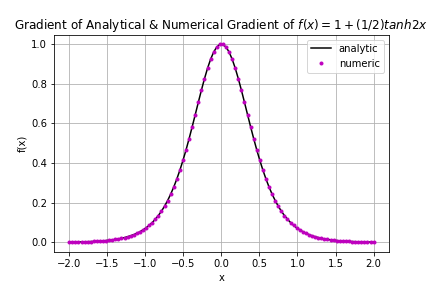
\includegraphics[width=0.7\textwidth]{analytic vs numeric.png}
		\caption{A plot of both the analytical and numerical gradients of the function $f(x) = 1 + \tanh(2x)$ }
		\label{fig:analytic vs numeric} 
	\end{center}
\end{figure} 



\section{Question 2}

The integrand of the gamma function 
\begin{equation}
	\Gamma(x) = \int_{0}^{\infty}x^{a-1}\exp^{-x} dx
\end{equation} 
is 
\begin{equation}
	f(x) = x^{a-1}\exp^{-x} 
\end{equation}

Plotting this function for different values of a on the interval x = [0, 5] yields the graph below.
\\
\begin{figure}[h]\begin{center} 
		\vspace{12pt}
		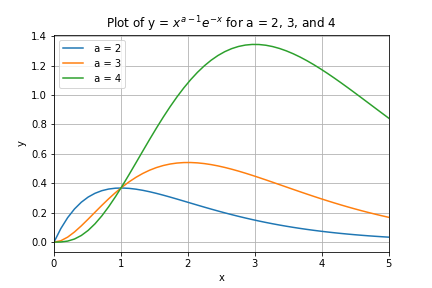
\includegraphics[width=0.6\textwidth]{gamma_integrand.png}
		\caption{A plot of the integrand $f(x) = x^{a-1}\exp^{-x} $ for a = 2, 3, and 4 }
		\label{fig:integrand} 
	\end{center}
\end{figure} 


For a function to be maximum, it's value when its first derivative is set to $0$. For the function 
\begin{equation}
	f(x) = x^{a-1}\exp^{-x} 
\end{equation}
we see that 
\begin{eqnarray}
	f'(x) &=& (a-1)x^{a-2}\exp^{-x} - x^{a-1}\exp^{-x} = 0 \\
	f'(x) &=& \frac{a-1}{x}x^{a-1}\exp^{-x} - x^{a-1}\exp^{-x} = 0\\
	      &=&  (\frac{a-1}{x} -1)x^{a-1}\exp^{-x} = 0
\end{eqnarray}
setting the coefficient to $0$ yields
\begin{eqnarray}
	\frac{a-1}{x} - 1 = 0 \\
	x = a - 1
\end{eqnarray}

% Question 2c
For a change in variables $z = \frac{x}{c + x}$, when solved analytically yields the value of  $z = \frac{1}{2}$ at $x = c$. Hence, $c = a -1$. The function is modified to 
\begin{equation}
	\Gamma(x) = \int_{0}^{\infty}\exp{(a-1)(\ln{x})}\exp^{-x} dx
\end{equation}

to prevent underflow and overflow.

Using the modified gamma function expression and change of variables, the function $gamma(a)$ was defined and $gamma(3/2)$ was calculated to have a value of 0.8862269613087213, which is approximates to be 0.866. Also, the values of gamma at a = 3, 6 and 10 were found to be 2.000000000000001, 119.99999999999999, and 362879.99999999994. These values are found to be consistent with the actual values, which are seen to have a formula of $(a-1)!$, with little errors arising from underflow or overflow from Python.




\section{Question 3}

Singular Value Decomposition can be used to make function fits to data. Here, a series of polynomials were tried and fitted against the original plot. In addition to that, a set of sines and cosines, forming a harmonic series, were also plotted against the data. The condition numbers $(w)$ were calculated in each case. The closer the condition number is to 1, the better the fit. 
\\
A plot of the original data obtained from the signal.dat file was plotted as shown in  \figurename{fig:signal data}
\begin{figure}[htp]\begin{center} 
		\vspace{12pt}
		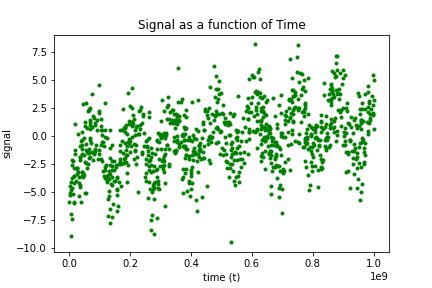
\includegraphics[width=0.6\textwidth]{signal data plot.png}
		\caption{A plot of signal as a function of time}
		\label{fig:signal data} 
	\end{center}
\end{figure} 
\\
A plot of the residuals in Figure \ref{fig:residual} show little difference in the original plot.
\begin{figure}[htp]\begin{center} 
		\vspace{12pt}
		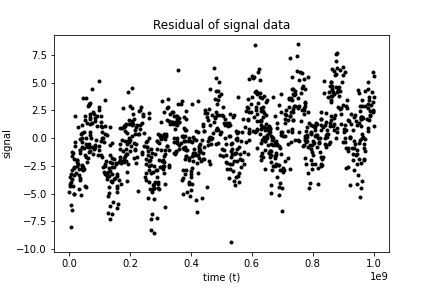
\includegraphics[width=0.6\textwidth]{residual.png}
		\caption{A plot of residual signal}
		\label{fig:residual} 
	\end{center}
\end{figure} 

A third order polynomial was fitted against the plot and plotted in Figure \ref{fig:third order polynomial fit}. The condition number was found to be 9.080721776290792e+24 of order 24 which is not appropriate.
\\

\begin{figure}[htp]\begin{center} 
		\vspace{12pt}
		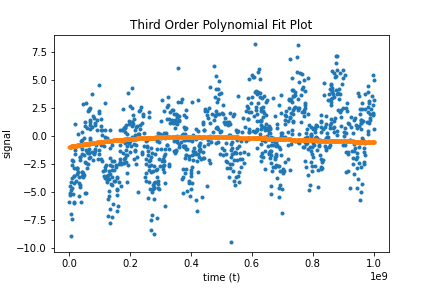
\includegraphics[width=0.6\textwidth]{third order poly.png}
		\caption{A plot of third order polynomial fit against the original data plot  }
		\label{fig:third order polynomial fit} 
	\end{center}
\end{figure} 

A higher order polynomial of order 11 was tested and plotted as shown in Figure \ref{fig:eleventh order polynomial fit}. The condition number was calculated as 6.633791010480661e+93, which is considerably worse than that of the third order polynomial fit.

\begin{figure}[htp]\begin{center} 
		\vspace{12pt}
		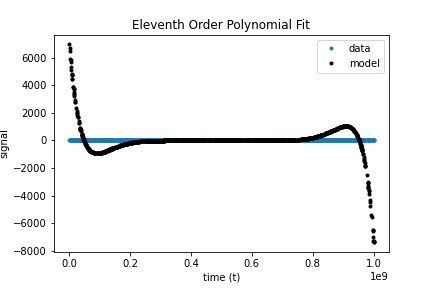
\includegraphics[width=0.6\textwidth]{eleventh order polynomial.png}
		\caption{A plot of an eleventh order polynomial fit against the original data plot }
		\label{fig:eleventh order polynomial fit} 
	\end{center}
\end{figure} 


It was revealed that higher order polynomials gave greater condition numbers and hence, worse fits. Any higher order polynomial returned an error with an infinite condition number. Hence, a plot of a first order polynomial was made as shown in Figure \ref{fig:first order polynomial fit} which revealed a condition number of 145696560.95949677 of order 10, which although bad, is better than the previous values. 
\\
Clearly, polynomials are not a good fit for the signal data.\\

\begin{figure}[htp]\begin{center} 
		\vspace{12pt}
		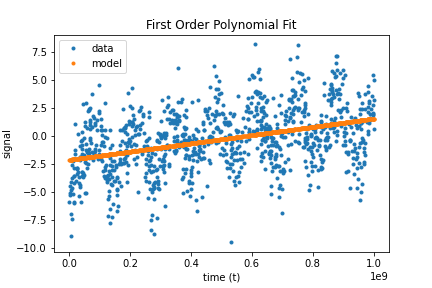
\includegraphics[width=0.6\textwidth]{first order Polynomial.png}
		\caption{A plot of a first order polynomial fit against the original data plot  }
		\label{fig:first order polynomial fit} 
	\end{center}
\end{figure} 


A set of cosines and sines were then used to fit the data as shown in Figure \ref{fig:harmonic sequence fit}. The harmonic sequence returned a condition number of 1.6822417943999717, which is proven to be the best choice for data of this type.

\begin{figure}[htp]\begin{center} 
		\vspace{12pt}
		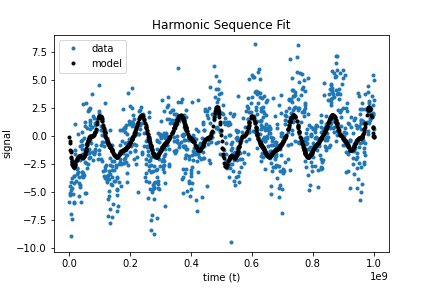
\includegraphics[width=0.6\textwidth]{harmonic sequence fit.png}
		\caption{A plot of a harmonic sequence fit against the original data plot  }
		\label{fig:harmonic sequence fit} 
	\end{center}
\end{figure} 










\end{document}